\documentclass[10pt]{article}
\usepackage[verbose, a4paper, hmargin=2.5cm, vmargin=2.5cm]{geometry}

\usepackage{fontspec}
\usepackage{ctex}
\usepackage{paratype}

\usepackage{amsmath}
\usepackage{amssymb}
\usepackage{amsfonts}
\usepackage{esint}
\usepackage{stmaryrd}

\usepackage[mathbf=sym]{unicode-math}
\setmainfont{STIX Two Text}
\setmathfont{STIX Two Math}

\setsansfont{Arial}
\setmonofont{Courier New}

\usepackage{makecell}
\usepackage{wasysym}
\usepackage{pifont}
\usepackage[export]{adjustbox}
\usepackage{graphicx}
\usepackage{mdframed}
\usepackage{booktabs,array,multirow}
\usepackage{tabularx}
\usepackage{hyperref}
\hypersetup{colorlinks=true, linkcolor=blue, filecolor=magenta, urlcolor=cyan,}
\urlstyle{same}
\usepackage[most]{tcolorbox}
\usepackage{tikz}

% 定义考点分析框
\newtcolorbox{analysisbox}[1][]{
  colback=blue!5,
  colframe=blue!50!black,
  fonttitle=\bfseries,
  title=#1,
  boxrule=0.5pt,
  arc=2mm,
  left=5pt,
  right=5pt,
  top=5pt,
  bottom=5pt
}

% 定义教学提示框
\newtcolorbox{tipbox}[1][]{
  colback=orange!5,
  colframe=orange!60!black,
  fonttitle=\bfseries,
  title=#1,
  boxrule=0.5pt,
  arc=2mm,
  left=5pt,
  right=5pt,
  top=5pt,
  bottom=5pt
}

\definecolor{mygray}{RGB}{240,240,240}
\tcbset{
  colback=mygray,
  boxrule=0pt,
}
\graphicspath{ {./images/} }
\newcommand{\HRule}{\begin{center}\rule{0.9\linewidth}{0.2mm}\end{center}}
\newcommand{\customfootnote}[1]{
  \let\thefootnote\relax\footnotetext{#1}
}
\newcommand{\lt}{\mathrel{<}}
\newcommand{\gt}{\mathrel{>}}
\newcommand*\circled[1]{\tikz[baseline=(char.base)]{\node[shape=circle,draw,inner sep=1.5pt] (char) {\small #1};}}
\setcounter{MaxMatrixCols}{256}

\begin{document}
\begin{center}
\Large\textbf{2026届崇明区高三下二模数学试卷}\\[0.5em]
\normalsize\textit{（教师版·带考点分析与教学评价）}
\end{center}

\section*{一、填空题}

1. 集合 \(A = \{ 2,4,6,8,{10}\} ,B = \left( {-1,6}\right)\) ，则 \(A \cap  B =\) \_\_\_\_.

\textbf{【答案】} \(\{ 2,4\}\)

\textbf{【解析】}由题意得, \(A \cap  B = \{ 2,4\}\) .

\begin{analysisbox}[考点分析]
\textbf{知识点}：集合的交集运算\\
\textbf{难度}：\(\star\) 基础题\\
\textbf{评价}：考查集合的基本运算，特别是离散集合与区间的交集。注意区分 \(\{2,4\}\) 与 \((2,4)\) 的不同。
\end{analysisbox}

2. 不等式 \(\left| {x - 1}\right|  < 2\) 的解为\_\_\_\_.

\textbf{【答案】} \(\{ x \mid   - 1 < x < 3\}\)

\textbf{【解析】} \(\because \left| {x - 1}\right|  < 2\) ,

\(\therefore  - 2 < x - 1 < 2\) ,解得 \(- 1 < x < 3\) ,

故不等式 \(\left| {x - 1}\right|  < 2\) 的解为 \(\{ x \mid   - 1 < x < 3\}\) .

\begin{analysisbox}[考点分析]
\textbf{知识点}：绝对值不等式\\
\textbf{难度}：\(\star\) 基础题\\
\textbf{评价}：绝对值不等式的基本解法，可等价转化为 \(-2 < x-1 < 2\)。学生易错点：忘记变号或解错区间端点。
\end{analysisbox}

3. 若复数 \(z\) 满足 \(\frac{z}{1 + \mathrm{i}} = \mathrm{i}\) ( \(\mathrm{i}\) 为虚数单位),则 \(z =\) \_\_\_\_.

\textbf{【答案】} \(- 1 + \mathrm{i}\)

\textbf{【解析】}因为 \(\frac{z}{1 + \mathrm{i}} = \mathrm{i}\) ,所以 \(z = \left( {1 + \mathrm{i}}\right) \mathrm{i} = \mathrm{i} + {\mathrm{i}}^{2} = \mathrm{i} - 1\) ,

所以 \(z =  - 1 + \mathrm{i}\)

\begin{analysisbox}[考点分析]
\textbf{知识点}：复数的四则运算\\
\textbf{难度}：\(\star\) 基础题\\
\textbf{评价}：复数乘法运算，注意 \(\mathrm{i}^2 = -1\)。此题也可通过分母有理化求解，考查学生的运算灵活性。
\end{analysisbox}

4. 已知向量 \(\overrightarrow{a} = \left( {k,2}\right)\) ， \(\overrightarrow{b} = \left( {2,1}\right)\) ，若 \(\overrightarrow{a}\bot \overrightarrow{b}\) ，则实数 \(k =\) \_\_\_\_.

\textbf{【答案】} -1

\textbf{【解析】}由 \(\overrightarrow{a} \bot  \overrightarrow{b}\) 得 \(\overrightarrow{a} \cdot  \overrightarrow{b} = 0\) ,

\(\therefore {2k} + 2 = 0,\therefore k =  - 1\) .

\begin{analysisbox}[考点分析]
\textbf{知识点}：平面向量的数量积与垂直条件\\
\textbf{难度}：\(\star\) 基础题\\
\textbf{评价}：向量垂直的充要条件是数量积为零。直接利用坐标公式 \(x_1x_2 + y_1y_2 = 0\) 即可求解。
\end{analysisbox}

5. 若 \(x > 0,y > 0\) ，且 \({xy} = 1\) ，则 \(x + {2y}\) 的最小值为\_\_\_\_.

\textbf{【答案】} \(2\sqrt{2}\)

\textbf{【解析】}由基本不等式可得 \(x + {2y} \geq  2\sqrt{2xy} = 2\sqrt{2}\) ,

当且仅当 \(x = {2y}\) ,即 \(x = \sqrt{2},y = \frac{\sqrt{2}}{2}\) 时等号成立,

所以 \(x + {2y}\) 的最小值为 \(2\sqrt{2}\) .

\begin{analysisbox}[考点分析]
\textbf{知识点}：基本不等式\\
\textbf{难度}：\(\star\) 基础题\\
\textbf{评价}：经典的基本不等式应用，注意配凑系数使乘积为定值。检验取等条件是得分关键。
\end{analysisbox}

6. 已知 \(\cos \theta  =  - \frac{3}{5}\) ，则 \(\cos {2\theta }\) 的值为\_\_\_\_.

\textbf{【答案】} \(- \frac{7}{25}\)

\textbf{【解析】}由 \(\cos \theta  =  - \frac{3}{5}\) ,则 \(\cos {2\theta } = 2{\cos }^{2}\theta  - 1 = 2 \times  \frac{9}{25} - 1 =  - \frac{7}{25}\) .

\begin{analysisbox}[考点分析]
\textbf{知识点}：二倍角公式\\
\textbf{难度}：\(\star\) 基础题\\
\textbf{评价}：二倍角公式的直接应用。选用 \(\cos 2\theta = 2\cos^2\theta - 1\) 最为简便，避免开方运算。
\end{analysisbox}

7. 从一副去掉大小王的 52 张扑克牌中随机抽取一张牌,事件 \(A\) 表示 ``取得的牌面是 \(A\) '',事件 \(B\) 表示``取得的牌的花色是黑桃''，则 \(P\left( {B \mid  A}\right)\) 为\_\_\_\_.

\textbf{【答案】} \(\frac{1}{4}\)

\textbf{【解析】} \(P\left( A\right)  = \frac{4}{52} = \frac{1}{13},P\left( {AB}\right)  = \frac{1}{52}\) ,故 \(P\left( {B \mid  A}\right)  = \frac{P\left( {AB}\right) }{P\left( A\right) } = \frac{\frac{1}{52}}{\frac{1}{13}} = \frac{1}{4}\) .

\begin{analysisbox}[考点分析]
\textbf{知识点}：条件概率\\
\textbf{难度}：\(\star\star\) 中档题\\
\textbf{评价}：条件概率的公式应用。也可直观理解：已知是A，则只可能是4种花色之一的A，故概率为1/4。考查学生的概率直觉。
\end{analysisbox}

8. 在 \(\bigtriangleup  {ABC}\) 中，角 \(A\) 、 \(B\) 、 \(C\) 所对的边长分别为 \(a\) 、 \(b\) 、 \(c\) . 若 \(A = {45}^{ \circ  }\) ， \(C = {30}^{ \circ  }\) ， \(c = \sqrt{2}\) ，则 \(a =\) \_\_\_\_.

\textbf{【答案】} 2

\textbf{【解析】}由正弦定理得 \(\frac{a}{\sin {45}^{ \circ  }} = \frac{\sqrt{2}}{\sin {30}^{ \circ  }}\) ,解得 \(a = \frac{\sqrt{2}\sin {45}^{ \circ  }}{\sin {30}^{ \circ  }} = 2\) .

\begin{analysisbox}[考点分析]
\textbf{知识点}：正弦定理\\
\textbf{难度}：\(\star\) 基础题\\
\textbf{评价}：正弦定理的直接应用，注意特殊角的三角函数值。\(\sin 45° = \frac{\sqrt{2}}{2}, \sin 30° = \frac{1}{2}\)。
\end{analysisbox}

9. 已知 \({\left( x - 1\right) }^{3} + {\left( x + 1\right) }^{4} = {x}^{4} + {a}_{1}{x}^{3} + {a}_{2}{x}^{2} + {a}_{3}x + {a}_{4}\) ,则 \({a}_{1} =\) \_\_\_\_.

\textbf{【答案】} 5

\textbf{【解析】}由题意, \({a}_{1}\) 为 \({x}^{3}\) 的系数, \({\left( x - 1\right) }^{3}\) 和 \({\left( x + 1\right) }^{4}\) 的展开式中都包含 \({x}^{3}\) 项,

故 \({a}_{1}{x}^{3} = {\mathrm{C}}_{3}^{0}{x}^{3} + {\mathrm{C}}_{4}^{1}{x}^{3} \times  1 = 5{x}^{3}\) ,

故 \({a}_{1} = 5\)

\begin{analysisbox}[考点分析]
\textbf{知识点}：二项式定理\\
\textbf{难度}：\(\star\star\) 中档题\\
\textbf{评价}：二项展开式特定项系数的求法。分别找出两个展开式中 \(x^3\) 的系数再相加。考查学生的细致程度，易漏掉其中一个展开式的贡献。
\end{analysisbox}

10. 如图,已知圆柱的一个截面边界是椭圆 \(\Gamma\) ,其中 \(\Gamma\) 的长轴 \({AC}\) 为该圆柱轴截面的对角线,短轴长等于圆柱底面直径的长. 将圆柱侧面沿母线 \({AB}\) 展开,则椭圆 \(\Gamma\) 在展开图中恰好为一个周期的三角函数图像. 若该段曲线是函数 \(y = 1 - \sqrt{3}\sin \frac{x}{2}\) 的图像的一部分,则椭圆 \(\Gamma\) 的离心率为\_\_\_\_.

\begin{center}
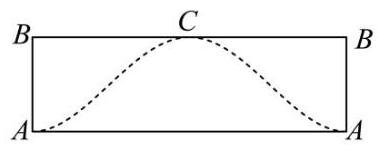
\includegraphics[max width=0.3\textwidth]{images/bo_d7ffhcs91nqc73erb3p0_1_1116_1751_378_152_0.jpg}
\end{center}

\textbf{【答案】} \(\frac{\sqrt{21}}{7}\)

\textbf{【解析】}函数 \(y = 1 - \sqrt{3}\sin \frac{x}{2}\) 的值域为 \(\left\lbrack  {1 - \sqrt{3},1 + \sqrt{3}}\right\rbrack\) ,最小正周期 \(T = \frac{2\pi }{\frac{1}{2}} = {4\pi }\) ,

依题意,圆柱的高 \(h = \left| {AB}\right|  = 2\sqrt{3}\) ,设圆柱的底面半径为 \(r\) ,则 \({2\pi r} = {4\pi }\) ,解得 \(r = 2\) ,

椭圆短轴长 \({2b} = {2r} = 4\) ,即 \(b = 2\) ,长轴长 \({2a} = \sqrt{{h}^{2} + {\left( 2r\right) }^{2}} = 2\sqrt{7}\) ,即 \(a = \sqrt{7}\) ,

所以椭圆的离心率 \(e = \frac{\sqrt{{a}^{2} - {b}^{2}}}{a} = \sqrt{1 - \frac{{b}^{2}}{{a}^{2}}} = \frac{\sqrt{21}}{7}\) .

\begin{analysisbox}[考点分析]
\textbf{知识点}：椭圆的几何性质、圆柱的展开图、三角函数的周期\\
\textbf{难度}：\(\star\star\star\) 难题\\
\textbf{评价}：本题是跨章节综合题，涉及立体几何与解析几何的深度融合。
\begin{itemize}
\item 关键突破点：理解圆柱展开后椭圆变成正弦曲线这一几何直观
\item 周期 \(4\pi\) 对应底面周长 \(2\pi r\)，由此求出 \(r=2\)
\item 振幅 \(\sqrt{3}\) 对应圆柱高的一半，由此求出 \(h=2\sqrt{3}\)
\item 最后用椭圆离心率公式求解
\end{itemize}
\textbf{教学建议}：建议画图演示圆柱展开过程，帮助学生建立空间想象。
\end{analysisbox}

\begin{tipbox}[教学提示]
本题是崇明卷的特色题，体现了上海高考数学``多想少算''的命题理念。学生需要在脑海中完成从三维到二维的转化，对空间想象能力要求较高。可类比：圆柱斜截面的椭圆在展开图上是正弦曲线，这是工程制图中的重要原理。
\end{tipbox}

11. 设 \({f}_{1}\left( x\right)  = \sin x,{f}_{2}\left( x\right)  = \cos \left( {x + \frac{\pi }{6}}\right)\) . 若对任意 \(t \in  \mathbf{R}\) ,存在 \(i \in  \{ 1,2\}\) 使得函数 \(y = {f}_{i}\left( x\right)\) 在区间 \(\left\lbrack  {t,t + a}\right\rbrack  \left( {a > 0}\right)\) 上是单调函数，则实数 \(a\) 的取值范围是\_\_\_\_.

\textbf{【答案】} \((0,\frac{\pi }{3}\rbrack\)

\textbf{【解析】} \({f}_{1}\left( x\right)  = \sin x\) ,由正弦函数的性质得到单调区间的分界点 \(x = \frac{\pi }{2} + {k\pi },k \in  \mathrm{Z}\) ,

相邻分界点间隔为 \(\pi\) ,因此每个单调区间的长度为 \(\pi\) ;

\({f}_{2}\left( x\right)  = \cos \left( {x + \frac{\pi }{6}}\right)\) ,令 \(x + \frac{\pi }{6} = {l\pi },l \in  \mathrm{Z}\) ,则 \(x = {l\pi } - \frac{\pi }{6},l \in  \mathrm{Z}\) ,

故单调区间的分界点 \(x = {k\pi } - \frac{\pi }{6},\;k \in  \mathrm{Z}\) ,

相邻分界点间隔为 \(\pi\) ,因此每个单调区间的长度为 \(\pi\) .

两类分界点合并排序,可发现它们交替排列,相邻两个不同类型的分界点的间隔交替为 \(\frac{\pi }{3}\) 和 \(\frac{2\pi }{3}\) ,

所以两类分界点之间的最小距离为 \(\frac{\pi }{3}\) ,所以 \(a \leq  \frac{\pi }{3}\) ,又 \(a > 0\) ,所以 \(a\) 的取值范围是 \(\left( {0,\frac{\pi }{3}}\right\rbrack\) .

\begin{analysisbox}[考点分析]
\textbf{知识点}：三角函数的单调性、逻辑量词（任意与存在）\\
\textbf{难度}：\(\star\star\star\) 难题\\
\textbf{评价}：本题是函数性质与逻辑推理的综合题。
\begin{itemize}
\item 核心难点：理解``对任意 \(t\)，存在 \(i\)''的逻辑含义——无论从哪里开始取区间，两个函数中至少有一个在该区间单调
\item 解题关键：找出两个函数单调分界点的分布规律
\item \(\sin x\) 的分界点：\(\frac{\pi}{2} + k\pi\)
\item \(\cos(x+\frac{\pi}{6})\) 的分界点：\(k\pi - \frac{\pi}{6}\)
\item 两类分界点交替排列，最小间隔为 \(\frac{\pi}{3}\)
\end{itemize}
\textbf{常见错误}：学生容易混淆``任意''和``存在''的顺序，或者无法找到两类分界点的相对位置关系。
\end{analysisbox}

\begin{tipbox}[教学提示]
这道题可以引导学生画出两个函数的单调分界点在数轴上的分布图，直观理解``无论从哪里开始，总能找到一个函数单调''的几何意义。建议用数轴演示分界点的交错排列，帮助学生理解最小间隔 \(\frac{\pi}{3}\) 的由来。
\end{tipbox}

12. 已知首项为 1 的等比数列 \(\left\{  {a}_{n}\right\}\) 满足对任意的正整数 \(m,n\) 都有 \(\left| {{a}_{m} - {a}_{n}}\right|  \leq  \frac{1}{3}\left| {m - n}\right|\) ,则等比数列 \(\left\{  {a}_{n}\right\}\) 的公比 \(q\) 的取值范围是\_\_\_\_.

\textbf{【答案】} \(\frac{2}{3} \leq  q \leq  1\)

\textbf{【解析】}由题意可得 \({a}_{n} = {a}_{1}{q}^{n - 1} = {q}^{n - 1}\) ,取 \(k = m - 1 \in  \mathbf{N}\) ,

当 \(n = 1\) 时,有 \(\left| {{a}_{m} - {a}_{n}}\right|  = \left| {{q}^{k} - 1}\right|  \leq  \frac{1}{3}k\) ,

当 \(k = 1\) 时,有 \(\left| {q - 1}\right|  \leq  \frac{1}{3}\) ,故 \(\frac{2}{3} \leq  q \leq  \frac{4}{3}\) ;

若 \(\left| q\right|  > 1\) ,则当 \(k \rightarrow   + \infty\) 时,指数函数增速会大于一次函数,

故 \(\left| {{q}^{k} - 1}\right|  \leq  \frac{1}{3}k\) 不可能恒成立,故 \(\left| q\right|  \leq  1\) ;

综上可得 \(\frac{2}{3} \leq  q \leq  1\) ;

下证充分性: 当 \(\frac{2}{3} \leq  q \leq  1\) 时,不妨设 \(m \geq  n\) ,则 \({a}_{m} \leq  {a}_{n}\) ,

故需满足 \({a}_{n} - {a}_{m} \leq  \frac{1}{3}\left( {m - n}\right)\) ,即 \({a}_{n} + \frac{1}{3}n \leq  {a}_{m} + \frac{1}{3}m\) ,

令 \({b}_{n} = {q}^{n - 1} + \frac{1}{3}n\) ,则只需满足数列 \(\left\{  {b}_{n}\right\}\) 为非递减数列即可,

\({b}_{n + 1} - {b}_{n} = {q}^{n} + \frac{1}{3}n + \frac{1}{3} - {q}^{n - 1} - \frac{1}{3}n = {q}^{n} - {q}^{n - 1} + \frac{1}{3} = {q}^{n - 1}\left( {q - 1}\right)  + \frac{1}{3},\)

由 \(\frac{2}{3} \leq  q \leq  1\) ,则 \(q - 1 \in  \left\lbrack  {-\frac{1}{3},0}\right\rbrack  ,{q}^{n - 1} \leq  1\) ,

则 \({b}_{n + 1} - {b}_{n} = {q}^{n - 1}\left( {q - 1}\right)  + \frac{1}{3} \geq   - \frac{1}{3} + \frac{1}{3} = 0\) ,

故数列 \(\left\{  {b}_{n}\right\}\) 为非递减数列,

即 \(\frac{2}{3} \leq  q \leq  1\) 时符合题意.

\begin{analysisbox}[考点分析]
\textbf{知识点}：等比数列、不等式恒成立、函数增长速度比较\\
\textbf{难度}：\(\star\star\star\star\) 压轴题\\
\textbf{评价}：本题是崇明卷填空压轴题，难度较大，分必要性证明和充分性证明两部分。
\begin{itemize}
\item \textbf{必要性}（求范围）：
  \begin{itemize}
  \item 取特殊值 \(n=1, k=1\) 得到 \(\frac{2}{3} \leq q \leq \frac{4}{3}\)
  \item 利用指数函数与一次函数增长速度的比较，排除 \(|q| > 1\)
  \item 得到 \(\frac{2}{3} \leq q \leq 1\)
  \end{itemize}
\item \textbf{充分性}（验证范围）：
  \begin{itemize}
  \item 构造辅助数列 \({b}_{n} = {q}^{n - 1} + \frac{1}{3}n\)
  \item 证明该数列非递减，从而原不等式成立
  \end{itemize}
\end{itemize}
\textbf{命题亮点}：将数列问题转化为函数单调性问题，体现了上海高考对数学思想方法的重视。
\end{analysisbox}

\begin{tipbox}[教学提示]
本题是上海高考数学典型的``压轴填空题''风格，对学生的综合数学素养要求很高。建议在讲解时：
\begin{enumerate}
\item 先引导学生理解题意：等比数列相邻项的差被线性控制
\item 必要性部分强调``必要条件''的思想——原条件对所有 \(m,n\) 成立，则对特定值也成立
\item 充分性部分的构造法技巧性强，可向学生强调辅助函数的构造思路
\end{enumerate}
\end{tipbox}

\section*{二、单选题}

13. 在空间内, 异面直线所成角的取值范围是( )

A. \(\left( {0,\frac{\pi }{2}}\right)\) B. \(\left( {0,\frac{\pi }{2}}\right\rbrack\) C. \(\left\lbrack  {0,\frac{\pi }{2}}\right)\) D. \(\left\lbrack  {0,\frac{\pi }{2}}\right\rbrack\)

\textbf{【答案】}B

\textbf{【解析】}由异面直线所成角的定义可知,过空间一点分别作相应直线的平行线,两条相交直线所成的直角或锐角为异面直线所成角,所以两条异面直线所成角的取值范围是 \(\left( {0,\frac{\pi }{2}}\right\rbrack\) ,

故选 B.

\begin{analysisbox}[考点分析]
\textbf{知识点}：异面直线所成角的定义\\
\textbf{难度}：\(\star\) 基础题\\
\textbf{评价}：考查基本概念。注意区分：
\begin{itemize}
\item 异面直线：不平行也不相交，所以夹角不能为 0
\item 所成角定义为锐角或直角，所以最大为 \(\frac{\pi}{2}\)
\end{itemize}
\end{analysisbox}

14. 下列函数中,在 \(\mathbf{R}\) 上为严格增函数的是( )

A. \(y = {x}^{2}\) B. \(y = \left| x\right|\) C. \(y = \sin x\) D. \(y = {x}^{3}\)

\textbf{【答案】}D

\textbf{【解析】}对于 \(\mathrm{A},y = {x}^{2}\) 是定义在 \(\mathbf{R}\) 上的偶函数,

在区间 \(\left( {-\infty ,0}\right)\) 上单调递减,在区间 \(\left( {0, + \infty }\right)\) 上单调递增,故 \(\mathrm{A}\) 不符合题意;

对于 \(\mathrm{B},y = \left| x\right|\) 是定义在 \(\mathbf{R}\) 上的偶函数,

在区间 \(\left( {-\infty ,0}\right)\) 上单调递减,在区间 \(\left( {0, + \infty }\right)\) 上单调递增,故 \(\mathrm{B}\) 不符合题意;

对于 \(\mathrm{C},y = \sin x\) 是定义在 \(\mathbf{R}\) 上的周期函数,

在区间 \(\left\lbrack  {-\frac{\pi }{2} + {2k\pi },\frac{\pi }{2} + {2k\pi }}\right\rbrack  ,k \in  \mathbf{Z}\) 上单调递增,在区间 \(\left\lbrack  {\frac{\pi }{2} + {2k\pi },\frac{3\pi }{2} + {2k\pi }}\right\rbrack  ,k \in  \mathbf{Z}\) 上单调递减,故 \(\mathrm{C}\) 不符合题意;

对于 \(\mathrm{D},\;y = {x}^{3}\) 在 \(\mathbf{R}\) 上为严格增函数,故 \(\mathrm{D}\) 符合题意.

\begin{analysisbox}[考点分析]
\textbf{知识点}：基本初等函数的单调性\\
\textbf{难度}：\(\star\) 基础题\\
\textbf{评价}：考查常见函数的单调性。\(y=x^3\) 是R上的严格增函数，这是学生容易忽视的知识点（容易误以为在0处``平''了）。实际上 \(y' = 3x^2 \geq 0\) 且仅在孤立点处为0，不影响整体严格递增。
\end{analysisbox}

15. 已知 \(A\left( {-a,0}\right) ,B\left( {a,0}\right) ,{l}_{1} : {ax} - y = 0,{l}_{2} : {ax} + y = 0\) ,其中 \(a > 1\) ,点 \(P\) 为平面内一点,记点 \(P\) 到 \({l}_{1}\) , \({l}_{2}\) 的距离分别为 \({d}_{1},{d}_{2}\) ,则下列条件中能使点 \(P\) 的轨迹为椭圆的是 ( )

A. \(\left| {PA}\right|  + \left| {PB}\right|  = {2a}\) B. \({\left| PA\right| }^{2} + {\left| PB\right| }^{2} = 4{a}^{2}\)

C. \({d}_{1}^{2} + {d}_{2}^{2} = 4{a}^{2}\) D. \({d}_{1} + {d}_{2} = {4a}\)

\textbf{【答案】}C

\textbf{【解析】}对于 \(\mathrm{A}\) ,因为 \(\left| {PA}\right|  + \left| {PB}\right|  = {2a} = \left| {AB}\right|\) ,所以 \(P\) 点轨迹为线段 \({AB}\) ,故 \(\mathrm{A}\) 错误;

对于 \(\mathrm{B}\) ,设 \(P\left( {x,y}\right)\) ,则由 \({\left( x + a\right) }^{2} + {y}^{2} + {\left( x - a\right) }^{2} + {y}^{2} = 4{a}^{2} \Rightarrow  {x}^{2} + {y}^{2} = {a}^{2}\) ,所以 \(P\) 点轨迹为圆,故 \(\mathrm{B}\) 错误;

对于 \(\mathrm{C}\) ,由 \({\left( \frac{\left| ax - y\right| }{\sqrt{{a}^{2} + 1}}\right) }^{2} + {\left( \frac{\left| ax + y\right| }{\sqrt{{a}^{2} + 1}}\right) }^{2} = 4{a}^{2} \Rightarrow  {a}^{2}{x}^{2} + {y}^{2} = 2{a}^{2}\left( {{a}^{2} + 1}\right)\) ,

因为 \(a > 1\) ,方程可化为 \(\frac{{x}^{2}}{2\left( {{a}^{2} + 1}\right) } + \frac{{y}^{2}}{2{a}^{2}\left( {{a}^{2} + 1}\right) } = 1\) ,所以 \(P\) 点轨迹为椭圆,故 \(\mathrm{C}\) 正确;

对于 \(\mathrm{D}\) ,由 \(\frac{\left| ax - y\right| }{\sqrt{{a}^{2} + 1}} + \frac{\left| ax + y\right| }{\sqrt{{a}^{2} + 1}} = {4a} \Rightarrow  \left| {{ax} - y}\right|  + \left| {{ax} + y}\right|  = {4a}\sqrt{{a}^{2} + 1}\) ,

\circled{1}  当 \({ax} - y \geq  0\) 且 \({ax} + y \geq  0\) ,即 \(- {ax} \leq  y \leq  {ax}\) 时,

去绝对值可得 \({ax} - y + {ax} + y = {4a}\sqrt{{a}^{2} + 1}\) ,即 \(x = 2\sqrt{{a}^{2} + 1}\) ,

此时结合约束条件 \(- {2a}\sqrt{{a}^{2} + 1} \leq  y \leq  {2a}\sqrt{{a}^{2} + 1}\) 可知点 \(P\) 的轨迹为垂直于 \(x\) 轴的线段;

\circled{2}  当 \({ax} - y \geq  0\) 且 \({ax} + y < 0\) ,即 \(y <  - {ax}\) 且 \(y \leq  {ax}\) ,

去绝对值可得 \({ax} - y - {ax} - y = {4a}\sqrt{{a}^{2} + 1}\) ,即 \(y =  - {2a}\sqrt{{a}^{2} + 1}\) ,

此时结合约束条件 \(- 2\sqrt{{a}^{2} + 1} \leq  x < 2\sqrt{{a}^{2} + 1}\) 可知点 \(P\) 的轨迹为垂直于 \(y\) 轴的线段;

\circled{3}  当 \({ax} - y < 0\) 且 \({ax} + y < 0\) ，即 \(y <  - {ax}\) 且 \(y > {ax}\) ，

去绝对值可得 \(- {ax} + y - {ax} - y = {4a}\sqrt{{a}^{2} + 1}\) ,即 \(x =  - 2\sqrt{{a}^{2} + 1}\) ,

此时结合约束条件 \(- {2a}\sqrt{{a}^{2} + 1} < y < {2a}\sqrt{{a}^{2} + 1}\) 可知点 \(P\) 的轨迹为垂直于 \(x\) 轴的线段;

\circled{4}  当 \({ax} - y < 0\) 且 \({ax} + y \geq  0\) ,即 \(y > {ax}\) 且 \(- {ax} \leq  y\) ,

去绝对值可得 \(- {ax} + y + {ax} + y = {4a}\sqrt{{a}^{2} + 1}\) ,即 \(y = {2a}\sqrt{{a}^{2} + 1}\) ,

此时结合约束条件 \(- 2\sqrt{{a}^{2} + 1} \leq  x < 2\sqrt{{a}^{2} + 1}\) 可知点 \(P\) 的轨迹为垂直于 \(y\) 轴的线段;

综上可知 \(P\) 点轨迹为四条线段,故 \(\mathrm{D}\) 错误.

\begin{analysisbox}[考点分析]
\textbf{知识点}：轨迹方程、椭圆的定义、点到直线距离\\
\textbf{难度}：\(\star\star\star\) 难题\\
\textbf{评价}：本题是解析几何综合题，四个选项分别对应四种不同的轨迹类型，需要逐一验证。
\begin{itemize}
\item 选项A：椭圆定义是到两定点距离之和为常数（且大于两定点间距离），此处等于 \(|AB|\)，退化为线段
\item 选项B：化简后为 \(x^2 + y^2 = a^2\)，是圆
\item 选项C：化简后为椭圆的标准方程，注意 \(a > 1\) 保证分母为正且不相等
\item 选项D：涉及绝对值方程，需要分类讨论，最终轨迹是四条线段组成的菱形
\end{itemize}
\end{analysisbox}

\begin{tipbox}[教学提示]
本题选项D的化简过程较为繁琐，涉及四种情况的分类讨论。在课堂讲解时，可以：
\begin{enumerate}
\item 先快速排除A、B两个明显错误的选项
\item 验证C为正确答案后即可停止（考试策略）
\item 如时间充裕，可详细讲解D的化简，展示绝对值方程处理技巧
\end{enumerate}
\end{tipbox}

16. 已知函数 \(y = f\left( x\right) ,x \in  \mathbf{R}\) . 定义集合 \(M = \left\{  {{x}_{0} \mid  \text{ 对任意的 }x > {x}_{0}\text{ ,都有 }f\left( x\right)  \leq  f\left( {x}_{0}\right) }\right\}\) . 对于所有使得 \(M = \left\lbrack  {-1,2}\right\rbrack\) 的函数 \(y = f\left( x\right)\) ,有以下两个命题:  \circled{1} 存在函数 \(y = f\left( x\right)\) 在 \(x =  - 2\) 处取极小值;  \circled{2} 存在函数 \(y = f\left( x\right)\) 图像是连续曲线. 下列判断正确的是( )

A.  \circled{1}  \circled{2} 都真 B.  \circled{1} 真\circled{2} 假 C.  \circled{1} 假\circled{2} 真 D.  \circled{1}  \circled{2} 都假

\textbf{【答案】}A

\textbf{【解析】}根据题意可知集合 \(M\) 为函数 \(y = f\left( x\right)\) 的非严格单调递增区间,

不妨令函数 \(f\left( x\right)  =  - \frac{1}{3}{x}^{3} - \frac{3}{2}{x}^{2} - {2x}\) ,易知 \({f}^{\prime }\left( x\right)  =  - {x}^{2} - {3x} - 2 =  - \left( {x + 1}\right) \left( {x + 2}\right)\) ,

因此当 \(x \in  \left( {-2, - 1}\right)\) 时， \({f}^{\prime }\left( x\right)  > 0\) ，当 \(x \in  \left( {-\infty , - 2}\right)\) 或 \(\left( {-1, + \infty }\right)\) 时， \({f}^{\prime }\left( x\right)  < 0\) ，

可知 \(f\left( x\right)\) 在 \(\left( {-2, - 1}\right)\) 上单调递增,在 \(\left( {-\infty , - 2}\right)\) 和 \(\left( {-1, + \infty }\right)\) 上单调递减,

此时函数 \(f\left( x\right)  =  - \frac{1}{3}{x}^{3} - \frac{3}{2}{x}^{2} - {2x}\) 满足在 \(M = \left\lbrack  {-1,2}\right\rbrack\) 上单调递减，满足题意，

即存在函数 \(y = f\left( x\right)\) 在 \(x =  - 2\) 处取极小值,且是连续曲线,因此 \circled{1}  \circled{2} 都真.

\begin{analysisbox}[考点分析]
\textbf{知识点}：函数单调性、极值、集合的描述法\\
\textbf{难度}：\(\star\star\star\star\) 压轴题\\
\textbf{评价}：本题是选择压轴题，核心难点在于理解集合 \(M\) 的定义。
\begin{itemize}
\item 集合 \(M = [-1, 2]\) 的几何意义：函数在 \([-1, 2]\) 上单调递减（非严格），且这是最大的这样的区间
\item 关键突破：理解``对任意 \(x > x_0\) 都有 \(f(x) \leq f(x_0)\)''等价于``函数在 \([x_0, +\infty)\) 上单调递减''
\item 构造实例：取三次函数 \(f(x) = -\frac{1}{3}x^3 - \frac{3}{2}x^2 - 2x\)
  \begin{itemize}
  \item 求导得 \(f'(x) = -(x+1)(x+2)\)
  \item 单调性：在 \((-\infty, -2)\) 递减，\((-2, -1)\) 递增，\((-1, +\infty)\) 递减
  \item 由此可知 \(M = [-1, 2]\)（需要验证端点）
  \item \(x = -2\) 是极小值点，函数连续
  \end{itemize}
\end{itemize}
\end{analysisbox}

\begin{tipbox}[教学提示]
这是一道非常``上海风格''的函数题，强调对概念的理解而非计算量。建议讲解时：
\begin{enumerate}
\item 先花充足时间解读集合 \(M\) 的定义，可画图示意
\item 引导学生思考：什么样的函数会有 \(M = [-1, 2]\)？
\item 三次函数是最佳选择，因为有明确的单调区间分界点
\item 强调``存在性''问题只需要构造一个例子即可
\end{enumerate}
\end{tipbox}

\section*{三、解答题}

17. 如图，在直三棱柱 \({ABC} - {A}_{1}{B}_{1}{C}_{1}\) 中， \({AB} = {BC} = \sqrt{2},{AC} = {A{A}_{1}} = 2\) ，且 \(D,E\) 分别是 \({AC},{A}_{1}{C}_{1}\) 的中点.

\begin{center}
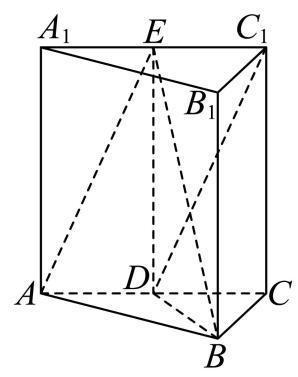
\includegraphics[max width=0.2\textwidth]{images/bo_d7ffhcs91nqc73erb3p0_5_1200_1616_298_377_0.jpg}
\end{center}

(1)证明: \(D{C}_{1}//\) 平面 \({ABE}\) ；

(2)求三棱锥 \({C}_{1} - {ABE}\) 的体积.

\textbf{【答案】}(1)见解析; (2) \(\frac{1}{3}\)

\textbf{【解析】}(1) 由直三棱柱性质可得 \({A}_{1}{C}_{1} = {AC},{A}_{1}{C}_{1}//{AC}\) ,

由 \(D,E\) 分别是 \({AC},{A}_{1}{C}_{1}\) 的中点,则 \({C}_{1}E = {AD},{C}_{1}E//{AD}\) ,

则四边形 \({AD}{C}_{1}E\) 是平行四边形,故 \(D{C}_{1}//{AE}\) ,

又 \({AE} \subset\) 平面 \({ABE},D{C}_{1} \not\subset\) 平面 \({ABE}\) ,故 \(D{C}_{1}//\) 平面 \({ABE}\) ;

(2)由 \({AB} = {BC} = \sqrt{2},{AC} = 2\) ，则 \({A{B}^{2}} + {B{C}^{2}} = {A{C}^{2}}\) ，

故 \(\bigtriangleup  {ABC}\) 为等腰直角三角形，则点 \(D\) 到 \({AB}\) 的距离为 \(\frac{1}{2}{BC} = \frac{\sqrt{2}}{2}\) ，

则点 \(E\) 到 \({A}_{1}{B}_{1}\) 的距离为 \(d = \frac{\sqrt{2}}{2}\) ,

由 \(E\) 为 \({A}_{1}{C}_{1}\) 的中点,则点 \({A}_{1}\) 与点 \({C}_{1}\) 到平面 \({ABE}\) 的距离相等,

故 \({V}_{{C}_{1} - {ABE}} = {V}_{{A}_{1} - {ABE}} = {V}_{E - {A}_{1}{BA}} = \frac{1}{3}{S}_{\bigtriangleup {A}_{1}{BA}} \cdot  d = \frac{1}{3} \times  \frac{1}{2} \times  2 \times  \sqrt{2} \times  \frac{\sqrt{2}}{2} = \frac{1}{3}\) .

\begin{analysisbox}[考点分析]
\textbf{知识点}：空间直线与平面的平行关系、三棱锥体积\\
\textbf{难度}：\(\star\star\) 中档题\\
\textbf{评价}：立体几何基础题，第(1)问考查线面平行的证明，第(2)问考查体积计算。
\begin{itemize}
\item 第(1)问思路：通过构造平行四边形证明线线平行，进而推出线面平行
\item 第(2)问关键点：
  \begin{itemize}
  \item 识别 \(\triangle ABC\) 为等腰直角三角形
  \item 利用等体积法转换顶点：\(V_{C_1-ABE} = V_{E-A_1BA}\)
  \item 点 \(E\) 到平面 \(A_1BA\) 的距离等于点 \(C_1\) 到该平面距离的一半
  \end{itemize}
\end{itemize}
\textbf{计算技巧}：等体积法是求三棱锥体积的常用技巧，通过转换顶点简化计算。
\end{analysisbox}

\begin{tipbox}[教学提示]
这是一道标准的立体几何基础题，适合作为解答题第一题。讲解时可强调：
\begin{enumerate}
\item 线面平行的证明路径：线线平行 $\Rightarrow$ 线面平行
\item 找平行关系时，中点往往暗示中位线或平行四边形
\item 等体积法的灵活应用，选择最容易计算的组合
\end{enumerate}
\end{tipbox}

18. 2025 年 11 月, 教育部等五部门联合印发《关于实施学生体质强健计划的意见》, 明确要求``中小学生每天综合体育活动时间不少于 2 小时''. 某学校为了解政策落实情况及其对学生视力的影响，随机抽取了 100 名学生进行每周累计体育活动时长的调查, 得到如下频率分布表:

\begin{center}
\adjustbox{max width=\textwidth}{
\begin{tabular}{|c|c|c|c|c|c|}
\hline
每周活动总时长 (单位:时) & \(\lbrack 0,7)\) & \(\lbrack 7,{14})\) & \(\lbrack {14},{21})\) & \(\lbrack {21},{28})\) & [28,35] \\
\cline{1-6}
频率 & 0.15 & 0.25 & 0.35 & 0.15 & 0.1 \\
\cline{1-6}
\hline
\end{tabular}
}
\end{center}

同时，对这 100 名学生的视力进行了检查，将视力达到 5.0 及以上定为``视力良好''，低于 5.0 定为``视力一般''，得到如下 \(2 \times  2\) 列联表 (部分数据缺失):

\begin{center}
\adjustbox{max width=\textwidth}{
\begin{tabular}{|c|c|c|c|}
\hline
\phantom{X} & 视力良好 & 视力一般 & 合计 \\
\cline{1-4}
活动时间达标 (不少于 14 小时) & 40 & \phantom{X} & \phantom{X} \\
\cline{1-4}
活动时间未达标 (低于 14 小时) & \phantom{X} & 30 & \phantom{X} \\
\cline{1-4}
合计 & \phantom{X} & \phantom{X} & 100 \\
\cline{1-4}
\hline
\end{tabular}
}
\end{center}

(1)从活动时长在 \(\left\lbrack  {0,7}\right)\) 和 \(\left\lbrack  {{28},{35}}\right\rbrack\) 的学生中，按比例分层随机抽样抽取 5 人进行座谈. 若从文 5 人中随机抽取 2 人，设 \(X\) 为抽取的 2 人中活动时长在 \(\left\lbrack  {{28},{35}}\right\rbrack\) 的人数，求 \(X\) 的分布列和数学期望 \(E\left\lbrack  X\right\rbrack\) ；

(2)依据 \(\alpha  = {0.05}\) 的独立性检验，判断是否有 95\%的把握认为``视力情况''与``体育活动时长是否达标''有关. 参考公式及数据:

\circled{1} \({\chi }^{2} = \frac{n{\left( ad - bc\right) }^{2}}{\left( {a + b}\right) \left( {c + d}\right) \left( {a + c}\right) \left( {b + d}\right) }\) ，其中 \(n = a + b + c + d\) .

\circled{2} \(P\left( {{\chi }^{2} \geq  {6.635}}\right)  \approx  {0.01}\) ， \(P\left( {{\chi }^{2} \geq  {5.024}}\right)  \approx  {0.025}\) ， \(P\left( {{\chi }^{2} \geq  {3.841}}\right)  \approx  {0.05}\) ， \(P\left( {{\chi }^{2} \geq  {2.706}}\right)  \approx  {0.1}\) .

\textbf{【答案】}(1)

\begin{center}
\adjustbox{max width=\textwidth}{
\begin{tabular}{|c|c|c|c|}
\hline
\(X\) & 0 & 1 & 2 \\
\cline{1-4}
\(P\) & \(\frac{3}{10}\) & \(\frac{3}{5}\) & \(\frac{1}{10}\) \\
\cline{1-4}
\hline
\end{tabular}
}
\end{center}

\(E\left( X\right)  = {0.8}\) ; (2)有 95\%的把握认为``视力情况''与``体育活动时长是否达标''有关.

\textbf{【解析】}(1) 由于 \(\left\lbrack  {0,7}\right)\) 和 \(\left\lbrack  {{28},{35}}\right\rbrack\) 频率分别为 \({0.15},{0.1},\frac{0.15}{0.1} = \frac{3}{2}\) ,

则按比例分层随机抽样,抽取 5 人进行座谈,有 3 人来自 \(\lbrack 0,7),2\) 人来自 \(\lbrack {28},{35}\rbrack\) ,

由题意 \(X\) 的可能取值为0,1,2,

\(P\left( {X = 0}\right)  = \frac{{\mathrm{C}}_{3}^{2}}{{\mathrm{C}}_{5}^{2}} = \frac{3}{10},\)

\(P\left( {X = 1}\right)  = \frac{{\mathrm{C}}_{3}^{1}{\mathrm{C}}_{2}^{1}}{{\mathrm{C}}_{5}^{2}} = \frac{3}{5},\)

\(P\left( {X = 2}\right)  = \frac{{\mathrm{C}}_{2}^{2}}{{\mathrm{C}}_{5}^{2}} = \frac{1}{10},\)

所以 \(X\) 的分布列是:

\begin{center}
\adjustbox{max width=\textwidth}{
\begin{tabular}{|c|c|c|c|}
\hline
\(X\) & 0 & 1 & 2 \\
\cline{1-4}
\(P\) & \(\frac{3}{10}\) & \(\frac{3}{5}\) & \(\frac{1}{10}\) \\
\cline{1-4}
\hline
\end{tabular}
}
\end{center}

\(E\left( X\right)  = 0 \times  \frac{3}{10} + 1 \times  \frac{3}{5} + 2 \times  \frac{1}{10} = {0.8}.\)

(2)由题意活动时间达标人数为 \({100} \times  \left( {{0.35} + {0.15} + {0.1}}\right)  = {60}\) ,

活动时间未达标人数为 \({100} \times  \left( {{0.15} + {0.25}}\right)  = {40}\) ,

故列联表如下:

\begin{center}
\adjustbox{max width=\textwidth}{
\begin{tabular}{|c|c|c|c|}
\hline
\phantom{X} & 视力良好 & 视力一般 & 合计 \\
\cline{1-4}
活动时间达标 (不少于 14 小时) & 40 & 20 & 60 \\
\cline{1-4}
活动时间未达标 (低于 14 小时) & 10 & 30 & 40 \\
\cline{1-4}
合计 & 50 & 50 & 100 \\
\cline{1-4}
\hline
\end{tabular}
}
\end{center}

零假设 \({H}_{0}\) : ``视力情况''与``体育活动时长是否达标''无关.

根据列联表数据,计算 \({\chi }^{2} = \frac{{100}{\left( {40} \times  {30} - {20} \times  {10}\right) }^{2}}{\left( {{40} + {20}}\right) \left( {{10} + {30}}\right) \left( {{40} + {10}}\right) \left( {{20} + {30}}\right) } = \frac{100}{6} \approx  {16.667} > {3.841}\) ,

根据小概率值 \(\alpha  = {0.05}\) 的独立性检验,判断 \({H}_{0}\) 不成立,

所以有 95\%的把握认为``视力情况''与``体育活动时长是否达标''有关.

\begin{analysisbox}[考点分析]
\textbf{知识点}：分层抽样、超几何分布、独立性检验（\(\chi^2\) 检验）\\
\textbf{难度}：\(\star\star\) 中档题\\
\textbf{评价}：统计综合题，结合时事背景（学生体质强健计划），体现数学应用价值。
\begin{itemize}
\item 第(1)问：分层抽样 + 超几何分布
  \begin{itemize}
  \item 分层比例：\([0,7)\) 与 \([28,35]\) 频率比为 \(0.15:0.1 = 3:2\)
  \item 抽取 5 人，则 3 人来自前者，2 人来自后者
  \item \(X\) 服从超几何分布，计算分布列和期望
  \end{itemize}
\item 第(2)问：独立性检验
  \begin{itemize}
  \item 根据频率分布计算达标人数：\(100 \times (0.35+0.15+0.1) = 60\)
  \item 补全列联表，计算 \(\chi^2\) 统计量
  \item 与临界值 \(3.841\) 比较，作出统计推断
  \end{itemize}
\end{itemize}
\end{analysisbox}

\begin{tipbox}[教学提示]
本题是应用题，建议讲解时：
\begin{enumerate}
\item 强调统计与现实的联系，引导学生关注社会热点
\item 分层抽样的比例计算要细心，建议画图辅助
\item 独立性检验的步骤要规范：建立假设 $\Rightarrow$ 计算统计量 $\Rightarrow$ 比较临界值 $\Rightarrow$ 作出推断
\item 注意结论的表述：``有 95\%的把握认为...有关''，而非``概率为 95\%''
\end{enumerate}
\end{tipbox}

19. 设函数 \(f\left( x\right)  = {x}^{2} - x + a\ln x,a \in  \mathbf{R}\) .

(1)若 \(a = 1\) ，求 \(f\left( x\right)\) 的图象在 \(x = 1\) 处的切线方程；

(2)若 \(f\left( x\right)  \geq  0\) 在 \(\lbrack 1, + \infty )\) 上恒成立，求 \(a\) 的取值范围；

\textbf{【答案】}(1) \({2x} - y - 2 = 0\) ; (2) \(\lbrack  - 1, + \infty )\)

\textbf{【解析】}(1) \(a = 1\) 时, \(f\left( x\right)  = {x}^{2} - x + \ln x\) ,对函数求导得 \({f}^{\prime }\left( x\right)  = {2x} - 1 + \frac{1}{x}\) .

所以 \({f}^{\prime }\left( 1\right)  = 2 - 1 + \frac{1}{1} = 2,f\left( 1\right)  = 0\) .

所以 \(f\left( x\right)\) 的图象在 \(x = 1\) 处的切线方程为 \(y - 0 = 2\left( {x - 1}\right)\) ,即 \({2x} - y - 2 = 0\) .

(2)由 \(f\left( x\right)  = {x}^{2} - x + a\ln x\) 得 \({f}^{\prime }\left( x\right)  = {2x} - 1 + \frac{a}{x} = \frac{2{x}^{2} - x + a}{x}\) .

因为 \(2{x}^{2} - x + a = 2{\left( x - \frac{1}{4}\right) }^{2} - \frac{1}{8} + a\) 在 \(\lbrack 1, + \infty )\) 上单调递增,所以 \({\left( 2{x}^{2} - x + a\right) }_{\text{ min }} = 1 + a\) .

若 \(a \geq   - 1\) ,则 \({f}^{\prime }\left( x\right)  \geq  0\) 在 \(\lbrack 1, + \infty )\) 上恒成立,所以 \(f\left( x\right)\) 在 \(\lbrack 1, + \infty )\) 上单调递增,

又 \(f\left( 1\right)  = 0\) ,所以 \(f\left( x\right)  \geq  0\) 在 \(\lbrack 1, + \infty )\) 上恒成立,

若 \(a <  - 1\) ,令 \({f}^{\prime }\left( x\right)  = 0\) 得 \(x = \frac{1 - \sqrt{1 - {8a}}}{4}\) 或 \(x = \frac{1 + \sqrt{1 - {8a}}}{4}\) ,且 \(\frac{1 - \sqrt{1 - {8a}}}{4} < 0,\frac{1 + \sqrt{1 - {8a}}}{4} > 1\) .

当 \(x \in  \left( {1,\frac{1 + \sqrt{1 - {8a}}}{4}}\right)\) 时, \({f}^{\prime }\left( x\right)  < 0,f\left( x\right)\) 单调递减,

所以 \(f\left( x\right)  < f\left( 1\right)  = 0\) ,与 \(f\left( x\right)  \geq  0\) 在 \(\lbrack 1, + \infty )\) 上恒成立矛盾,

综上所述, \(a\) 的取值范围是 \(\lbrack  - 1, + \infty )\) .

\begin{analysisbox}[考点分析]
\textbf{知识点}：导数的几何意义（切线）、利用导数研究函数的单调性和最值、恒成立问题\\
\textbf{难度}：\(\star\star\star\) 难题\\
\textbf{评价}：函数与导数综合题，是上海高考解答题的常规题型。
\begin{itemize}
\item 第(1)问：基础求切线
  \begin{itemize}
  \item 求导数得斜率 \(f'(1) = 2\)
  \item 点斜式写出切线方程
  \end{itemize}
\item 第(2)问：恒成立问题，分类讨论
  \begin{itemize}
  \item 思路：求导 $\Rightarrow$ 分析单调性 $\Rightarrow$ 找最小值 $\Rightarrow$ 保证最小值 $\geq 0$
  \item 关键：分析 \(g(x) = 2x^2 - x + a\) 在 \([1, +\infty)\) 上的符号
  \item 分类讨论临界点：\(a = -1\)
    \begin{itemize}
    \item \(a \geq -1\) 时，\(f'(x) \geq 0\)，函数递增，\(f(x) \geq f(1) = 0\)
    \item \(a < -1\) 时，存在递减区间，导致 \(f(x) < 0\)，矛盾
    \end{itemize}
  \end{itemize}
\end{itemize}
\end{analysisbox}

\begin{tipbox}[教学提示]
本题是导数综合题的标准套路，建议讲解时强调：
\begin{enumerate}
\item 恒成立问题的转化策略：转化为求函数最值
\item 分类讨论的依据：导数的符号由分子 \(2x^2 - x + a\) 决定，其在 \([1, +\infty)\) 的最小值为 \(1+a\)
\item 当 \(1+a < 0\)（即 \(a < -1\)）时，导数有零点，函数先减后增，最小值可能小于0
\item 强调端点值 \(f(1) = 0\) 的特殊意义
\end{enumerate}
\end{tipbox}

20. 已知椭圆 \(C : \frac{{x}^{2}}{4} + \frac{{y}^{2}}{3} = 1\) .

(1)求椭圆 \(C\) 的离心率 \(e\) ；

(2)已知椭圆右顶点为 \(A\) ，设点 \(M\) 为 \(y\) 轴正半轴上一点，点 \(P\) 为椭圆 \(C\) 上的一点. 若 \(\overrightarrow{AP} = 2\overrightarrow{PM}\) ，求点 \(M\) 的坐标;

(3)已知 \(G\left( {\frac{5}{2},0}\right)\) ,过点 \(R\left( {4,0}\right)\) 的直线交椭圆 \(C\) 于 \(D,E\) 两点,直线 \({DG}\) 交直线 \(x = 1\) 于点 \(H\) ,证明: \({EH} \bot  y\) 轴.

\textbf{【答案】} \(\left( 1\right) \frac{1}{2};\left( 2\right) \left( {0,\sqrt{6}}\right) ;\left( 3\right)\) 见解析.

\textbf{【解析】}(1) 记椭圆 \(C : \frac{{x}^{2}}{4} + \frac{{y}^{2}}{3} = 1\) 的长轴长为 \({2a}\) ,短轴长为 \({2b}\) ,焦距为 \({2c}\) ,

则 \(a = 2,b = \sqrt{3},c = \sqrt{{a}^{2} - {b}^{2}} = 1\) ,所以离心率 \(e = \frac{c}{a} = \frac{1}{2}\) .

(2)由题知， \(A\left( {2,0}\right)\) ，设 \(M\left( {0,m}\right) ,m > 0\) ， \(P\left( {{x}_{P},{y}_{P}}\right)\) ，

因为 \(\overrightarrow{AP} = \left( {{x}_{P} - 2,{y}_{P}}\right) ,\overrightarrow{PM} = \left( {-{x}_{P},m - {y}_{P}}\right) ,\overrightarrow{AP} = 2\overrightarrow{PM}\) ,

所以 \(\left( {{x}_{P} - 2,{y}_{P}}\right)  = 2\left( {-{x}_{P},m - {y}_{P}}\right)\) ,得 \({x}_{P} = \frac{2}{3},{y}_{P} = \frac{2m}{3}\) ,

代入椭圆方程得 \(\frac{1}{9} + \frac{4{m}^{2}}{27} = 1\) ，解得 \(m = \sqrt{6}\) (负根舍去)

(3)易知，当直线 \({DE}\) 斜率为 0 时， \(D,E\) 为长轴端点， \(H\) 与右焦点重合，满足题意；

设直线 \({DE}\) 的方程为 \(x = {ny} + 4,D\left( {{x}_{1},{y}_{1}}\right) ,E\left( {{x}_{2},{y}_{2}}\right)\) ,

联立 \(\left\{  \begin{array}{l} \frac{{x}^{2}}{4} + \frac{{y}^{2}}{3} = 1 \\  x = {ny} + 4 \end{array}\right.\) 得: \(\left( {3{n}^{2} + 4}\right) {y}^{2} + {24ny} + {36} = 0\) ,

由 \(\Delta  = {\left( {24}n\right) }^{2} - 4\left( {3{n}^{2} + 4}\right)  \times  {36} = {144}\left( {{n}^{2} - 4}\right)  > 0\) 得 \(n <  - 2\) 或 \(n > 2\) ,

则 \({y}_{1} + {y}_{2} = \frac{-{24n}}{3{n}^{2} + 4},{y}_{1}{y}_{2} = \frac{36}{3{n}^{2} + 4}\) ,

所以 \(3\left( {{y}_{1} + {y}_{2}}\right)  =  - {2n}{y}_{1}{y}_{2}\) ,则 \({y}_{2} = \frac{-3{y}_{1}}{3 + {2n}{y}_{1}}\) ,

设 \(H\left( {1,h}\right)\) ,因为 \(D,H,G\) 三点共线,则 \(\overrightarrow{DH}//\overrightarrow{HG},\overrightarrow{DH} = \left( {1 - {x}_{1},h - {y}_{1}}\right) ,\overrightarrow{HG} = \left( {\frac{3}{2}, - h}\right)\) ,

所以 \(- h\left( {1 - {x}_{1}}\right)  = \frac{3}{2}\left( {h - {y}_{1}}\right)\) ,则 \(h = \frac{3{y}_{1}}{5 - 2{x}_{1}} = \frac{3{y}_{1}}{5 - 2\left( {n{y}_{1} + 4}\right) } = \frac{-3{y}_{1}}{3 + {2n}{y}_{1}}\) ,

所以 \(h = {y}_{2}\) ,所以 \({EH} \bot  y\) 轴.

\begin{analysisbox}[考点分析]
\textbf{知识点}：椭圆的标准方程与几何性质、向量共线、直线与椭圆的位置关系\\
\textbf{难度}：\(\star\star\star\) 难题\\
\textbf{评价}：解析几何综合题，是上海高考的传统压轴题型，计算量较大。
\begin{itemize}
\item 第(1)问：基础求离心率，\(e = \frac{c}{a} = \frac{1}{2}\)
\item 第(2)问：向量定比分点问题
  \begin{itemize}
  \item 由 \(\overrightarrow{AP} = 2\overrightarrow{PM}\) 得 \(P\) 分 \(AM\) 的比为 \(2:1\)
  \item 用定比分点公式或向量坐标运算求出 \(P\) 坐标
  \item 代入椭圆方程求 \(m\)
  \end{itemize}
\item 第(3)问：定点定值问题的证明
  \begin{itemize}
  \item 设直线 \(DE: x = ny + 4\)（避免讨论斜率不存在）
  \item 联立椭圆，用韦达定理表示 \(y_1 + y_2, y_1y_2\)
  \item 利用 \(D,H,G\) 共线，求出 \(H\) 的纵坐标 \(h\)
  \item 目标是证明 \(h = y_2\)，即 \(EH \parallel x\) 轴（垂直于 \(y\) 轴）
  \item 关键是找到 \(y_1, y_2, n\) 之间的关系式
  \end{itemize}
\end{itemize}
\end{analysisbox}

\begin{tipbox}[教学提示]
第(3)问是难题，建议讲解时：
\begin{enumerate}
\item 强调设直线方程的技巧：设 \(x = ny + 4\) 比 \(y = k(x-4)\) 更简洁，避免斜率讨论
\item 韦达定理的应用要熟练，建议学生背诵：\(y_1+y_2 = -\frac{24n}{3n^2+4}, y_1y_2 = \frac{36}{3n^2+4}\)
\item 关键是发现关系式 \(3(y_1+y_2) = -2ny_1y_2\)，这在后续的化简中会用到
\item 共线条件的转化：利用斜率相等或向量共线
\item 这类``证明某直线垂直于某轴''的问题，通常转化为证明两点纵坐标相等
\end{enumerate}
\end{tipbox}

21. 函数 \(y = f\left( x\right) ,x \in  \mathbf{R}\) 是减函数,即对于任意的 \({x}_{1},{x}_{2} \in  \mathbf{R}\) ,当 \({x}_{1} < {x}_{2}\) 时,均有 \(f\left( {x}_{1}\right)  \geq  f\left( {x}_{2}\right)\) .

(1)若 \(f\left( x\right)  =  - {x}^{3} + {ax}\) ，求实数 \(a\) 的取值范围；

( 2 )是否存在函数 \(y = f\left( x\right)\) 是偶函数，且满足 \(f\left( {f\left( x\right) }\right)  = x\) 对所有 \(x \in  \mathbf{R}\) 成立？若存在，请举出一个满足条件的函数, 若不存在, 请说明理由;

(3) 设 \(g\left( x\right)  = \sin x\) ，已知函数 \(h\left( x\right)  = f\left( x\right)  + g\left( x\right)\) 是周期函数，求证: \(f\left( x\right)\) 为常值函数.

\textbf{【答案】}( 1 ) \(\left( {-\infty ,0\rbrack}\right)\) ; (2)不存在，见解析；(3)见解析

\textbf{【解析】}(1) \(f\left( x\right)\) 为减函数,则 \({f}^{\prime }\left( x\right)  =  - 3{x}^{2} + a \leq  0\) 即 \(a \leq  3{x}^{2}\) 恒成立,所以 \(a \leq  0\) .

(2)因为 \(f\left( x\right)\) 为减函数，取任意实数 \({x}_{1}\) ， \({x}_{2}\) ，设 \({x}_{1} < {x}_{2}\) ，则有 \(f\left( {x}_{1}\right)  \geq  f\left( {x}_{2}\right)\) ，

又 \(f\left( x\right)\) 为偶函数即有 \(f\left( x\right)  = f\left( {-x}\right)\) ,可得 \(f\left( {-{x}_{1}}\right)  \geq  f\left( {-{x}_{2}}\right)\) ,

同时根据单调性由 \(- {x}_{1} >  - {x}_{2}\) 可得 \(f\left( {-{x}_{1}}\right)  \leq  f\left( {-{x}_{2}}\right)\) ,所以 \(f\left( {-{x}_{1}}\right)  = f\left( {-{x}_{2}}\right)\)

即 \(f\left( {x}_{1}\right)  = f\left( {x}_{2}\right)\) 对任意实数 \({x}_{1},{x}_{2}\) 成立,所以 \(f\left( x\right)\) 为常值函数,设 \(f\left( x\right)  = C\) ,

则 \(f\left( {f\left( x\right) }\right)  = f\left( C\right)  = C\) ,

当 \(x \neq  C\) 时, \(f\left( {f\left( x\right) }\right)  = x\) 不成立,所以不存在满足条件的函数.

(3)设函数 \(h\left( x\right)\) 的正周期为 \(T\) 即对任意 \(x \in  \mathbf{R}\) 都有 \(f\left( x\right)  + g\left( x\right)  = f\left( {x + T}\right)  + g\left( {x + T}\right)\) ，

因为 \(x < x + T\) ,根据 \(f\left( x\right)\) 为减函数可知 \(f\left( x\right)  \geq  f\left( {x + T}\right)\) ,所以 \(g\left( x\right)  \leq  g\left( {x + T}\right)\) ,

那么有 \(g\left( {x + \pi }\right)  \leq  g\left( {x + \pi  + T}\right)\) ,因为 \(g\left( {x + \pi }\right)  = \sin \left( {x + \pi }\right)  =  - \sin x =  - g\left( x\right)\) ,

所以 \(- g\left( x\right)  \leq   - g\left( {x + T}\right)\) 即 \(g\left( x\right)  \geq  g\left( {x + T}\right)\) ,于是可得 \(g\left( x\right)  = g\left( {x + T}\right)\) ,从而 \(f\left( x\right)  = f\left( {x + T}\right)\) ,

而 \(f\left( x\right)\) 为减函数,所以 \(f\left( x\right)\) 在 \(\left\lbrack  {a,a + T}\right\rbrack\) 上为常值函数,其中 \(a\) 为任意实数,

所以 \(f\left( x\right)\) 在 \(\mathbf{R}\) 上为常值函数.

\begin{analysisbox}[考点分析]
\textbf{知识点}：函数单调性、奇偶性、周期性、函数方程\\
\textbf{难度}：\(\star\star\star\star\) 压轴题\\
\textbf{评价}：本题是崇明卷的压轴题，以``减函数''为主线，三问层层递进，考查函数性质的综合运用。
\begin{itemize}
\item 第(1)问：基础求参数范围
  \begin{itemize}
  \item \(f'(x) = -3x^2 + a \leq 0\) 恒成立
  \item \(a \leq 3x^2\) 的最小值，得 \(a \leq 0\)
  \end{itemize}
\item 第(2)问：存在性问题的逻辑推理
  \begin{itemize}
  \item 核心矛盾：减函数 + 偶函数 $\Rightarrow$ 常值函数
  \item 证明思路：设 \(x_1 < x_2\)，利用减函数得 \(f(x_1) \geq f(x_2)\)
  \item 利用偶函数得 \(f(-x_1) = f(x_1), f(-x_2) = f(x_2)\)
  \item 又 \(-x_1 > -x_2\)，利用减函数得 \(f(-x_1) \leq f(-x_2)\)
  \item 故 \(f(x_1) = f(x_2)\)，即 \(f\) 为常值函数
  \item 常值函数不满足 \(f(f(x)) = x\)，矛盾！
  \end{itemize}
\item 第(3)问：周期函数性质的深度运用
  \begin{itemize}
  \item 关键等式：\(f(x) + \sin x = f(x+T) + \sin(x+T)\)
  \item 利用 \(f\) 递减：\(f(x) \geq f(x+T)\)，推出 \(\sin x \leq \sin(x+T)\)
  \item 用 \(x+\pi\) 替换 \(x\)：\(-\sin x \leq -\sin(x+T)\)，即 \(\sin x \geq \sin(x+T)\)
  \item 故 \(\sin x = \sin(x+T)\)，进而 \(f(x) = f(x+T)\)
  \item 周期且递减 $\Rightarrow$ 常值函数
  \end{itemize}
\end{itemize}
\end{analysisbox}

\begin{tipbox}[教学提示]
这是一道非常精彩的函数综合题，体现了上海高考``重思维轻计算''的特点。建议讲解时：
\begin{enumerate}
\item 第(2)问是逻辑推理的经典题型，要引导学生体会``反证法''的思想：假设存在，推出矛盾
\item 第(3)问的技巧性很强，关键是利用 \(x+\pi\) 替换得到双向不等式
\item 可以向学生强调：这类题的结论往往具有一般性（如第2问的``减+偶=常值''，第3问的``递减+周期=常值''）
\item 建议布置变式练习：若 \(f\) 递增且 \(f+g\) 周期，结论如何？
\end{enumerate}
\end{tipbox}

\vfill
\begin{center}
\rule{0.5\textwidth}{0.4pt}\\[0.5em]
\textit{— 试卷解析结束 —}\\[0.3em]
\small 本解析版包含详细考点分析与教学评价，供教师备课参考
\end{center}

\end{document}
